{\fontsize{12pt}{22pt} \textbf{Gradient descent}\par}

\vspace{5mm}

$\ell$ the loss function to minimize:

$\theta_{t+1}=\theta_t - \alpha \nabla \ell$ \\

\begin{algorithm}
\caption{Global gradient descent}
\begin{algorithmic}
\State Loss function $\widehat{L}_n(\hat{f}_\omega(x))=\Sigma_{i=1}^n \mathcal{\ell}(\hat{f}_\omega(x),y)$
\State $E=1000$
\State $\epsilon$ = small value
\State $\omega_0$ = intial value in $t_0$
\While{$E > \epsilon$}
\State $\omega_{t+1}=\omega_t-\epsilon\Sigma_{i=1}^n\nabla_\omega{\mathcal{\ell}(\hat{f}_\omega(x),y)}$
\State Compute $E=L_n(\omega_{t+1})$
\EndWhile
\end{algorithmic}
\end{algorithm}


\begin{algorithm}
\caption{Stochastic gradient descent}
\begin{algorithmic}
\State Loss function $\widehat{L}_n(\hat{f}_\omega(x))=\Sigma_{i=1}^n \mathcal{\ell}(\hat{f}_\omega(x),y)$
\State $E=1000$
\State $\epsilon$ = small value
\State $\omega_0$ = intial value in $t_0$
\While{$E > \epsilon$}
\For{i = 1,...,n}
\State $\omega_{t+1}=\omega_t-\epsilon\nabla_\omega{\mathcal{\ell}(\hat{f}_\omega(x_i),y_i)}$
\State Compute $E=L_n(\omega_{t+1})$
\EndFor
\EndWhile
\end{algorithmic}
\end{algorithm}

\begin{algorithm}
\caption{Stochastic and random gradient descent}
\begin{algorithmic}
\State Loss function $\widehat{L}_n(\hat{f}_\omega(x))=\Sigma_{i=1}^n \mathcal{\ell}(\hat{f}_\omega(x),y)$
\State $E=1000$
\State $\epsilon$ = small value
\State $\omega_0$ = intial value in $t_0$
\While{$E > \epsilon$}
\For{i = 1,...,n}
\State Random draw of $i \in \{1,...,n\}$
\State $\omega_{t+1}=\omega_t-\epsilon\nabla_\omega{\mathcal{\ell}(\hat{f}_\omega(x_i),y_i)}$
\State Compute $E=L_n(\omega_{t+1})$
\EndFor
\EndWhile
\end{algorithmic}
\end{algorithm}

\vspace{30mm}

The main advantage of stochastic gradient is that it avoid computing the gradient descent on all the observations (greedy). However, in doing so, the gradient descent is subject to noise and can take longer to reach the optimum. \\

\textit{Note}: the gradient is the derivation w.r.t $\omega$

\textit{Note (stochastic and random gradient descent)}: the draw can be done with or without replacement. \\



\underline{Proof of the gradient descent formula}:

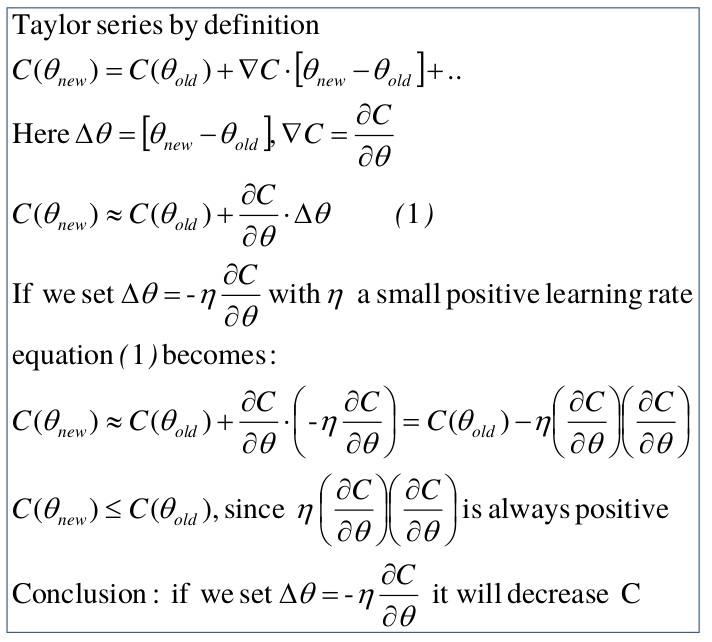
\includegraphics[scale=0.3]{../images/GradientDescent_proof.png}

(Idemia courses "DeepLearningTPT2018S1S2.pdf")

\vspace{5mm}
\underline{Learning rate optimization}
\vspace{5mm}

Note:

- one epoch = one forward pass and one backward pass of all the training examples.

- batch size = the number of training examples in one forward/backward pass. The higher the batch size, the more memory space needed.

- number of iterations = number of passes, each pass using [batch size] number of examples. To be clear, one pass = one forward pass + one backward pass.

\vspace{5mm}

\textit{Learning rate decay}

Simple idea: reduce the learning rate progressively.

E.g. $1/t$ decay:

$$\alpha_t=\frac{1}{(t+1)}$$

\vspace{5mm}
\textit{Momentum}

Momentum is a method that helps accelerate SGD in the relevant direction and reduce oscillations.

General idea:

$0 \le \gamma \le 1$

$M_{t_0}=x_0$

$M_{t_1}=\gamma M_{t_0} + x_1$

$M_{t_2}=\gamma M_{t_1} + x_2$

Let's develop $M_{t_2}$ to have a better view of momentum effect:

$M_{t_2} = \gamma (\gamma M_{t_0} + x_1) + x_2 = \gamma^2 x_0 + \gamma x_1 + x_2$

We can see that more importance is given to the most recent value ($x_2$) and the least to the past values.

\vspace{5mm}

In practice, $\gamma = 0.9$ gives good results.

\textbf{Advantage}: less dependent on noise

\vspace{5mm}
\textit{Adagrad - Adaptive Gradient Algorithm (2011)}

Divide the learning rate by "average" gradient:

$\theta_t = \theta_{t-1} - \frac{\alpha}{\sqrt{\Sigma_{i=0}^t(\nabla f_i^2)}}\nabla f$

\vspace{5mm}
\textit{RMSProp - Root Mean Squared Propagation}

Same as AdaGrad, but with an exponentially decaying average of past squared gradients.

$\theta_t = \theta_{t-1} - \frac{\alpha}{\sigma_{t-1}}\nabla f$

Where:

$\sigma_{t} = \sqrt{\alpha (\sigma_{t-1})^2+(1-\alpha)(\nabla f_t)^2}$


\vspace{5mm}
\textit{Adam - Adaptive moment estimation}

Adam = RMS + momentum => use of a exponential decaying average of past \underline{squared} gradients and past gradients

\vspace{5mm}